\section{Use Cases}

\subsection{Use Case Diagram}
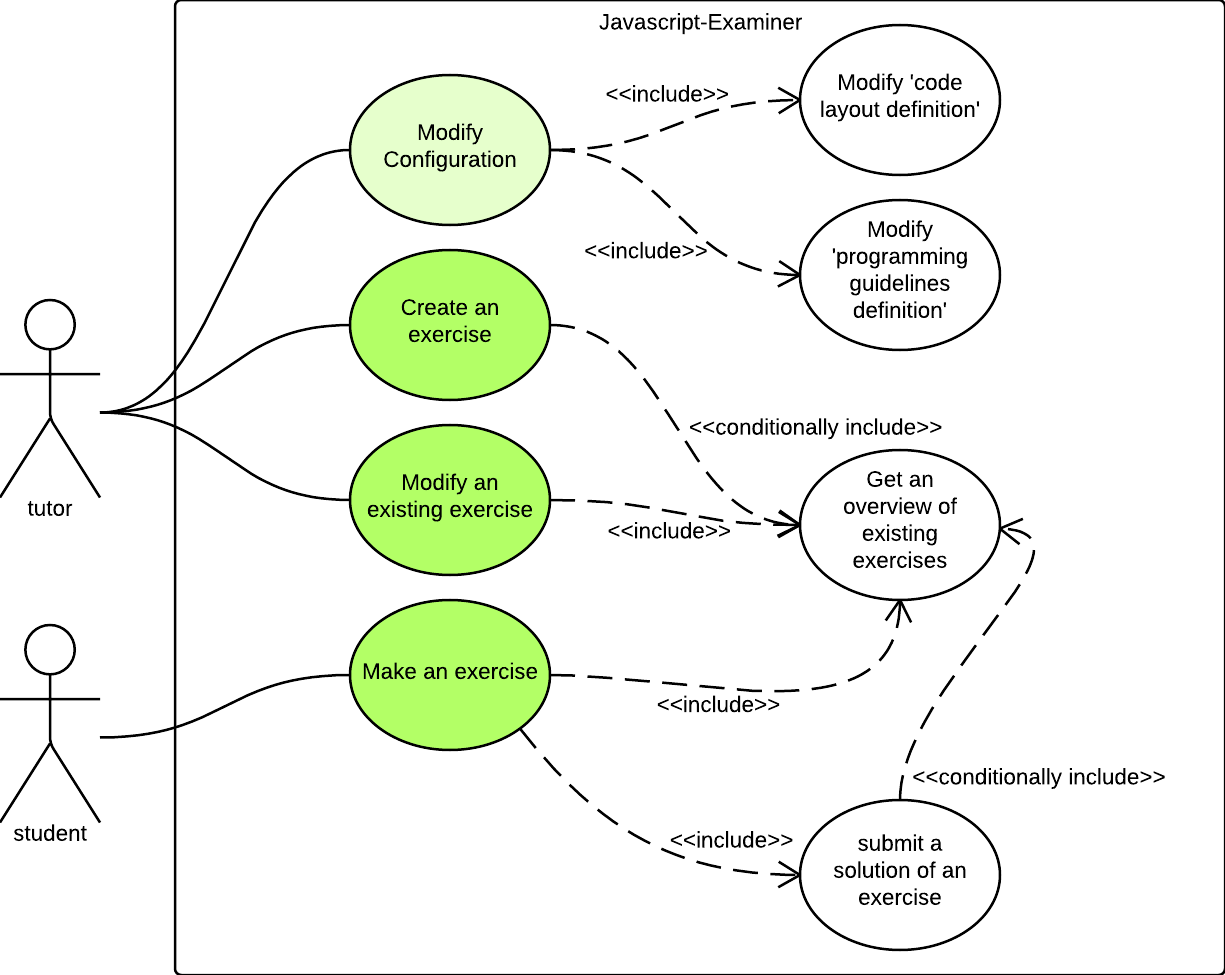
\includegraphics[scale=1.2]{diagrams-images/use-case-diagram}

\subsection{Main Use Cases}

\subsubsection{Create an Exercise}

\subsubsection{Modify an Exercise}

\subsubsection{Make an exercise}
\begin{mdframed} [rightmargin=-100pt]
\begin{description}
  \item[Scope] Javascript-Examiner
  \item[Level] user goal
  \item[Primary Actor] Student
  \item[Preconditions] There is at least 1 exercise available.
  \item[Success Guarantee] Student has received feedback on the submitted 
	solution.
  \item[Main Success Scenario] \mbox{}
	\begin{enumerate}
	  \item Student selects exercise from overview. \underline{Include: get
        an overview of available exercises}
	  \item Student requests exercise instruction.
	  \item System presents exercise instruction.
	  \item Student submits solution. \underline{Include: submit a solution of 
	    an exercise}
	  \item System presents feedback
	\end{enumerate}
\end{description}
\end{mdframed}

\subsubsection{Modify configuration}
\newpage
\subsection{Supporting Use Cases}

\subsubsection{Get an overview of existing exercises}
\begin{mdframed} [rightmargin=-100pt]
\begin{description}
  \item[Scope] Javascript-Examiner
  \item[Level] Subfunction
  \item[Primary Actor] Student, Tutor
  \item[Preconditions] Usecase \underline{make an exercise}, 
							   \underline{create an exercise} or
							   \underline{modify an exercise} initiated.
  \item[Success Guarantee] An overview of available exercises is 
    presented.
  \item[Main Success Scenario] \mbox{}
    \begin{enumerate} 
	  \item Student / Tutor requests overview of exercises
	  \item System presents overview of exercises
	\end{enumerate}
  \item[Extensions] \mbox{}
    \begin{enumerate}
	  \renewcommand{\labelenumi}{\theenumi a.}
	  \item Only a selection of the exercises is being requested:
		\begin{enumerate}[(1)]
		  \renewcommand{\labelenumii}{\theenumii .}
		  \item Student/Tutor provides a search string.
		  \item System presents the selection of exercises.
		\end{enumerate}
	\end{enumerate}
\end{description}
\end{mdframed}

\subsubsection{Submit the solution of an exercise}
\begin{mdframed} [rightmargin=-100pt]
\begin{description}
  \item[Scope] Javascript-Examiner
  \item[Level] Subfunction
  \item[Primary Actor] Student
  \item[Preconditions] Usecase \underline{make an exercise} initiated.
  \item[Success Guarantee] The solution has been submitted, the student has been
    provided with feedback.
  \item[Main Success Scenario] \mbox{}
    \begin{enumerate}
		\item Student requests submission of the solution.
		\item System requests the solution.
		\item Student submits the solution.
		\item System presents feedback on solution.
    \end{enumerate} 
  \item[Extensions] \mbox{}
	\begin{enumerate}
      \renewcommand{\labelenumi}{\theenumi a.}
	  \item The interaction with the system has been interupted:
		\begin{enumerate}[(1)]
		  \renewcommand{\labelenumii}{\theenumii .}
		  \item Student selects corresponding exercise from overview. \\
		    \underline{Include: get an overview of available exercises}
		  \item System shows options for selected exercise.
		  \item Student requests submission of the solution.
		\end{enumerate}
	\end{enumerate}
\end{description}
\end{mdframed}